\documentclass[a4paper]{compendium}
\usepackage[swedish]{babel}
\addto\captionsswedish{%
  \renewcommand{\appendixname}{Appendix}%
}
%TODO: Glossary
%http://tex.stackexchange.com/questions/5821/creating-a-standalone-glossary/5837#5837

\setlength{\columnsep}{16mm}

\title{
{\bf\Huge\sffamily  Programmering, grundkurs} 
\\ \vspace{2em}
{\sffamily  Kompendium}
}

%\author{Redaktör: Björn Regnell}
\date{EDAA45, Lp1-2, HT 2016 \\ 
Datavetenskap, LTH \\ 
Lunds Universitet  \\~\\
\url{http://cs.lth.se/pgk}}

\usepackage{pgffor}  %% http://stackoverflow.com/questions/2561791/iteration-in-latex
                     %  allows:  \foreach \n in {1,...,4}{ do something with \n }

\usepackage{framed}  %  allows:   \begin{framed}\end{framed}
%\newenvironment{Slide}[2][]
%  {\begin{framed}\setlist{noitemsep}\section*{#2}}
%  {\end{framed}}

\newcommand{\SlideHeading}[1]{\section*{#1}}

\usepackage[most]{tcolorbox}
\newenvironment{Slide}[2][]
  {\vspace{0.5em}\begin{tcolorbox}[%breakable, 
                                   enhanced]\setlist{noitemsep}\SlideHeading{#2}}
  {\end{tcolorbox}\vspace{0.5em}}

\newcommand{\Subsection}[1]{} %ignore slide sections
\newcommand{\SlideOnly}[1]{} %ignore slide font size

\newif\ifkompendium  % to allow conditional text in slides only showing up in compendium
\kompendiumtrue      % in slides: \kompendiumfalse
                

%!TEX encoding = UTF-8 Unicode
\newcommand{\ExeWeekONE}{expressions}
\newcommand{\LabWeekONE}{kojo}

\newcommand{\ExeWeekTWO}{programs}
\newcommand{\LabWeekTWO}{--}

\newcommand{\ExeWeekTHREE}{functions}
\newcommand{\LabWeekTHREE}{bugs}

\newcommand{\ExeWeekFOUR}{data}
\newcommand{\LabWeekFOUR}{pirates}

\newcommand{\ExeWeekFIVE}{sequences}
\newcommand{\LabWeekFIVE}{cards}

\newcommand{\ExeWeekSIX}{classes}
\newcommand{\LabWeekSIX}{turtlegraphics}

\newcommand{\ExeWeekSEVEN}{traits}
\newcommand{\LabWeekSEVEN}{turtlerace-team}

\newcommand{\ExeWeekEIGHT}{matching}
\newcommand{\LabWeekEIGHT}{chords-team}

\newcommand{\ExeWeekNINE}{matrices}
\newcommand{\LabWeekNINE}{maze}

\newcommand{\ExeWeekTEN}{sorting}
\newcommand{\LabWeekTEN}{surveydata-team}

\newcommand{\ExeWeekELEVEN}{scalajava}
\newcommand{\LabWeekELEVEN}{lthopoly-team}

\newcommand{\ExeWeekTWELVE}{threads}
\newcommand{\LabWeekTWELVE}{life}

\newcommand{\ExeWeekTHIRTEEN}{Uppsamling}
\newcommand{\LabWeekTHIRTEEN}{Projekt}

\newcommand{\ExeWeekFOURTEEN}{Extenta}
\newcommand{\LabWeekFOURTEEN}{--}


\begin{document}
\maketitle
%!TEX encoding = UTF-8 Unicode
%!TEX root = ../compendium.tex

\clearpage\null\thispagestyle{empty}
\vfill

{
\setlength{\parindent}{0pt}
\emph{Editor}: Björn Regnell \\ 

\emph{Contributors}: 
Björn Regnell, ...
\\

\emph{Home}: \url{https://cs.lth.se/pgk} \\ \newline

\emph{Repo}: \url{https://github.com/lunduniversity/introprog} \\ \newline

This manuscript is on-going work. Contributions are welcome! \\ 
\emph{Contact}: \url{bjorn.regnell@cs.lth.se}
\\ \newline

\emph{LICENCE}: CC BY-SA 4.0 \\
\url{http://creativecommons.org/licenses/by-sa/4.0/} \\
Please do \emph{not} distribute your solutions to lab assignments. 
\\ \newline
Copyright \copyright~Computer Science, LTH, Lund University. 2016. Lund. Sweden.\\
}
%!TEX encoding = UTF-8 Unicode
%!TEX root = ../compendium.tex

\ChapterUnnum{Framstegsprotokoll} 


\subsubsection*{Genomförda övningar}

\vspace{1em}\noindent 
{Till varje laboration hör en övning med uppgifter som utgör förberedelse inför labben. Du behöver minst behärska grundövningarna för att klara labben inom rimlig tid. Om du känner att du behöver öva mer på grunderna, gör då även extrauppgifterna. Om du vill fördjupa dig, gör fördjupningsuppgifterna som är på mer avancerad nivå. Genom att du kryssar för nedan vilka övningar du har gjort, blir det lättare för handledaren att förstå vilka förkunskaper du har inför labben.}

\newcommand{\TickBox}{\raisebox{-.50ex}{\Large$\square$}}
\newcommand{\ExeRow}[1]{\texttt{#1} & \TickBox  &  \TickBox &  \TickBox  \\ \addlinespace }

\begin{table}[h]
\centering
\vspace{2em}
\begin{tabular}{lccc}
\toprule \addlinespace 
{\sffamily\small Övning} & 
{\sffamily\small Grund} &	
{\sffamily\small Extra} &
{\sffamily\small Fördjupning}\\ \addlinespace \midrule \\[-0.7em]
\ExeRow{expressions}
\ExeRow{programs}
\ExeRow{functions}
\ExeRow{data}
\ExeRow{vectors}
\ExeRow{classes}
\ExeRow{traits}
\ExeRow{matching}
\ExeRow{matrices}
\ExeRow{sorting}
\ExeRow{scalajava}
\ExeRow{threads}
\bottomrule
\end{tabular}
\end{table}

\newpage

\subsubsection*{Godkända obligatoriska moment}

\vspace{1em}\noindent 
För att bli godkänd på laborationsuppgifterna och inlämningsuppgiften måste du lösa deluppgifterna och diskutera dina lösningar med en handledare. Denna diskussion är din möjlighet att få feedback på dina lösningar. Ta vara på den!
Se till att handledaren noterar när du blivit godkänd på detta blad, som är ditt kvitto. Spara detta blad tills du fått slutbetyg i kursen. 


\vspace{2.5em}\noindent Namn: \dotfill\\

\vspace{1em}\noindent Namnteckning: \dotfill\\

\newcommand{\LabRow}[1]{\\[-1.1em] \texttt{#1} & \dotfill &  \dotfill  \\ \addlinespace }

\begin{table}[h]
\centering
\vspace{1em}
\begin{tabular}{lcc}
\toprule \addlinespace 
{\sffamily\bfseries\small Lab} & {\sffamily\small Datum gk} &	{\sffamily\small Handledares namnteckning}\\ \addlinespace \midrule \\[-0.5em]
%!TEX encoding = UTF-8 Unicode
\LabRow{kojo}
\LabRow{bugs}
\LabRow{pirates}
\LabRow{cards}
\LabRow{turtlegraphics}
\LabRow{turtlerace-team}
\LabRow{chords-team}
\LabRow{maze}
\LabRow{surveydata-team}
\LabRow{lthopoly-team}
\LabRow{life}
\LabRow{Projekt}
%\toprule 
\addlinespace \midrule \addlinespace
{\sffamily\small {\bfseries Inlämningsuppgift} (välj en)	} & & \\ \addlinespace\addlinespace %\midrule
\texttt{( ) bank}  &  &  \\
\texttt{( ) mandelbrot} \\  
\texttt{( ) draw}  \\
\texttt{( ) egendefinerad}  \\
\textit{\small Om egen, ge kort beskrivning:}\\
%\dotfill  \\
\bottomrule
\end{tabular}
\end{table}
%!TEX encoding = UTF-8 Unicode
%!TEX root = ../compendium.tex


\ChapterUnnum{Förord} 

Programmering är inte bara ett sätt att ta makten över de människoskapade system som är förutsättningen för vårt moderna samhälle. Programmering är också ett kraftfullt verktyg för tanken. Med kunskap i programmeringens grunder kan du påbörja den livslånga läranderesa som det innebär att vara systemutvecklare och abstraktionskonstnär. Programmeringsspråk och utvecklingsverktyg kommer och går, men de grundläggande koncepten bakom \emph{all} mjukvara består: sekvens, alternativ, repetition och abstraktion. 

Detta kompendium utgör kursmaterial för en grundkurs i programmering, som syftar till att ge en solid bas för ingenjörsstudenter och andra som vill utveckla system med mjukvara. Materialet omfattar en termins studier på kvartsfart och förutsätter kunskaper motsvarande gymnasienivå i svenska, matematik och engelska. 

Kompendiet är framtaget för och av studenter och lärare, och distribueras som öppen källkod. Det får användas fritt så länge erkännande ges och eventuella ändringar publiceras under samma licens som ursprungsmaterialet. På kurshemsidan \href{http://cs.lth.se/pgk}{cs.lth.se/pgk} och i kursrepot \href{http://github.com/lunduniversity/introprog}{github.com/lunduniversity/introprog} finns instruktioner om hur du kan bidra till kursmaterialet.

Läromaterialet fokuserar på lärande genom praktiskt programmeringsarbete och innehåller övningar och laborationer som är organiserade i moduler. Varje modul har ett tema och en teoridel i form av föreläsningsbilder med tillhörande anteckningar. 

I kursen använder vi språken Scala och Java för att illustrera grunderna i imperativ och objektorienterad programmering, tillsammans med elementär funktionsprogrammering. Mer avancerad objektorientering och funktionsprogrammering lämnas till efterföljande fördjupningskurser. 

Den kanske viktigaste framgångsfaktorn vid studier i programmering är att bejaka din egen upptäckarglädje och experimentlusta. Det fantastiska med programmering är att dina egna intellektuella konstruktioner faktiskt \emph{gör} något som just \emph{du} har bestämt! Ta vara på det och prova dig fram genom att koda egna idéer -- det är kul när det funkar men minst lika lärorikt är felsökning, buggrättande och alla misslyckade försök som efter hårt arbete vänds till lyckade lösningar och/eller bestående lärdomar. 

Välkommen i programmeringens fascinerande värld och hjärtligt lycka till med dina studier!

\vspace{2em}\noindent\emph{LTH, Lund 2016}


\mainmatter
\tableofcontents

\part{Om kursen}      
%!TEX root = ../compendium.tex

\ChapterUnnum{Kursens arkitektur}

%!TEX encoding = UTF-8 Unicode
%!TEX root = ../lect-week01.tex

%%%%%%%%%%%%%%%%%%%%%%%%%%%%%%%%%%%%%%
\Subsection{Om kursen}

%%%

\begin{Slide}{Veckoöversikt}
\noindent\resizebox{0.9\columnwidth}{!}{
%!TEX encoding = UTF-8 Unicode
\begin{tabular}{l|l|l|l}
\textit{W} & \textit{Modul} & \textit{Övn} & \textit{Lab} \\ \hline \hline
W01 & Introduktion            & expressions & kojo            \\
W02 & Kodstrukturer           & programs    & --              \\
W03 & Funktioner, Objekt      & functions   & simplewindow    \\
W04 & Datastrukturer          & data        & textfiles       \\
W05 & Sekvensalgoritmer       & sequences   & cardgame        \\
W06 & Klasser, Likhet         & classes     & shapes          \\
W07 & Arv, Gränssnitt         & traits      & turtlerace-team \\
KS  & KONTROLLSKRIVN.         & --          & --              \\
W08 & Mönster, Undantag       & matching    & chords-team     \\
W09 & Matriser, Typparametrar & matrices    & maze            \\
W10 & Sökning, Sortering      & sorting     & surveydata-team \\
W11 & Scala och Java          & scalajava   & scalajava-team  \\
W12 & Trådar, Web, Android    & threads     & life            \\
W13 & Design                  & Uppsamling  & Inl.Uppg.       \\
W14 & Tentaträning            & Extenta     & --              \\
T   & TENTAMEN                & --          & --              \\
\end{tabular}

}
\end{Slide}

\ifkompendium
\noindent Kursen består av ett antal moduler med tillhörande teori, övningar och laborationer. Genom att göra övningarna bearbetar du teorin och förebereder dig inför laborationerna. När du klarat av  övningarna och laborationen i en modul är du redo att gå vidare till nästa modul.  
\fi

\begin{Slide}{Vad lär du dig?}
\begin{itemize}
\item Grundläggande principer för programmering:\\ Sekvens, Alternativ, Repetition, Abstraktion (SARA)\\$\implies$Inga förkunskaper i programmering krävs!
\item Konstruktion av algoritmer
\item Tänka i abstraktioner
\item Förståelse för flera olika angreppssätt: 
\begin{itemize}
\item \Emph{imperativ programmering}%: satser, föränderlighet
\item \Emph{objektorientering}%: inkapsling, återanvändning
\item \Emph{funktionsprogrammering}%: uttryck, oföränderlighet
\end{itemize}
\item Programspråken \Emph{Scala} och \Emph{Java}
\item Utvecklingsverktyg (editor, kompilator, utvecklingsmiljö)
\item Implementera, testa, felsöka
\end{itemize}
\end{Slide}

\begin{Slide}{Hur lär du dig?}
\begin{itemize}
\item Genom praktiskt \Alert{eget arbete}: \Emph{Lära genom att göra!}
\begin{itemize}
\item Övningar: applicera koncept på olika sätt
\item Laborationer: kombinera flera koncept till en helhet
\end{itemize}
\item Genom studier av kursens teori: \Emph{Skapa förståelse!}
\item Genom samarbete med dina kurskamrater: \Emph{Gå djupare!}
\end{itemize}
\end{Slide}


\begin{Slide}{Kurslitteratur}
\begin{minipage}{0.46\textwidth}
\centering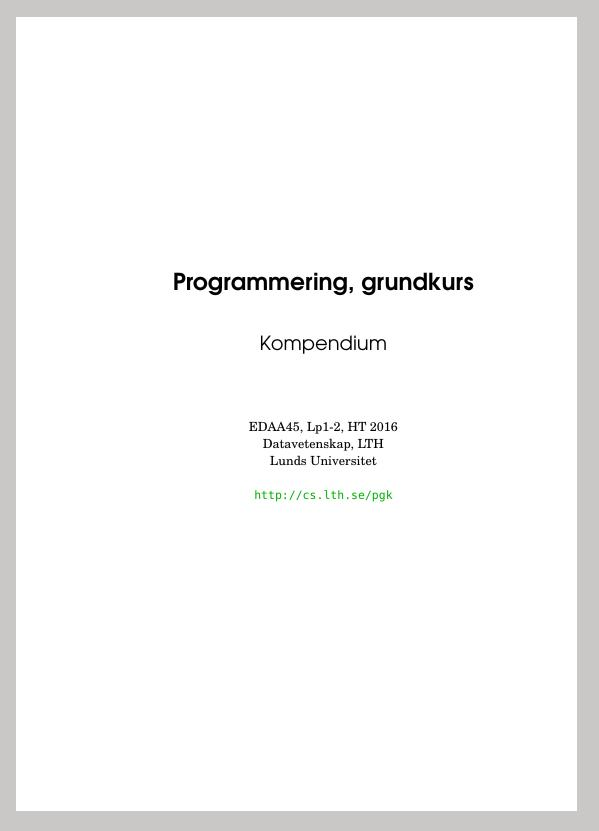
\includegraphics[width=0.45\textwidth]{../img/frontpage.jpg}
\begin{itemize}
\item \Emph{Kompendium} med föreläsningsanteckningar, övningar \& laborationer
\item Säljs på KFS \\\small\url{http://www.kfsab.se/}
\end{itemize}
\end{minipage}
\hskip2em\begin{minipage}{0.45\textwidth}
\Emph{\small Rekommenderade böcker}\\ 
\small För nybörjare:
\vskip0.2mm
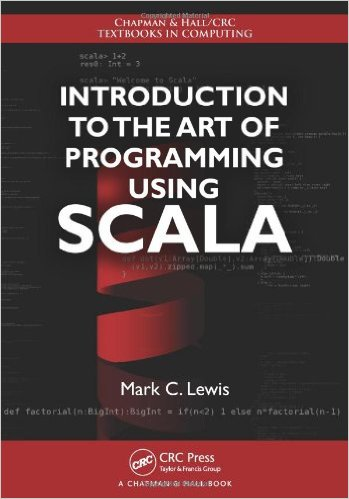
\includegraphics[width=0.35\textwidth]{../img/lewisbook.jpg}\hskip1mm
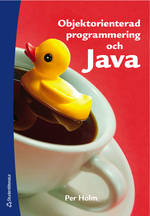
\includegraphics[width=0.35\textwidth]{../img/ankbok.jpg}

\noindent För de som redan kodat en del:
\vskip0.7mm
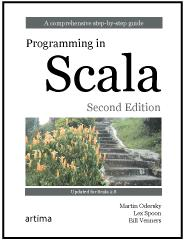
\includegraphics[width=0.4\textwidth]{../img/pinsbook.jpg}\hskip1mm

\includegraphics[width=0.42\textwidth]{../img/koffmanbook.jpg}
\end{minipage}
\end{Slide}

\ifkompendium\else
\begin{Slide}{Personal}
\begin{description}\small
\item [\bfseries Kursansvarig:] ~\\Björn Regnell, bjorn.regnell@cs.lth.se
\item [\bfseries Kurssekreterare:]  ~\\Lena Ohlsson \\Exp.tid 09.30 -- 11.30 samt 12.45 -- 13.30
\item [\bfseries Handledare:] ~\\
Maj	Stenmark,	Tekn. Lic., Doktorand\\
Gustav	Cedersjö,	Doktorand\\
Anton	Klarén,	D09\\
Maria	Priisalu	, D11\\
Anders	Buhl,	D13\\
Erik	Bjäreholt,	D13\\
Fatima	Abou Alpha,	D13\\
Cecilia	Lindskog,	D14\\
Emma	Asklund,	D14\\
\end{description}
\end{Slide}
\fi

\begin{Slide}{Kursmoment --- varför?}\SlideOnly{\footnotesize}
\begin{itemize}
\item \Emph{Föreläsningar}: skapa översikt, ge struktur, förklara teori, svara på frågor, motivera varför
\item \Emph{Övningar}: bearbeta teorin med avgränsade problem, grundövningar för alla, extraövningar om du behöver öva mer, fördjupningsövningar om du vill gå vidare, \Alert{förberedelse} inför laborationerna
\item \Emph{Laborationer}: lösa programmeringsproblem praktiskt, \Alert{obligatoriska} uppgifter; lösningar redovisas för handledare
\item \Emph{Resurstider}: få hjälp med övningar och laborationsförberedelser av handledare, fråga vad du vill
\item \Emph{Samarbetsgrupper}: grupplärande genom samarbete, hjälpa varandra 
\item \Emph{Kontrollskrivning}: \Alert{obligatorisk}, diagnostisk, kamraträttad; kan ge samarbetsbonuspoäng till tentan
\item \Emph{Individuell projektuppgift}: \Alert{obligatorisk}, du visar att du kan skapa ett större program självständigt; redovisas för handledare
\item \Emph{Tenta}: Skriftlig tentamen utan hjälpmedel, förutom  \href{http://fileadmin.cs.lth.se/cs/Education/EDA016/general/quickref-booklet.pdf}{snabbreferens}.
\end{itemize}
\end{Slide}

\ifkompendium\else
\begin{Slide}{Detta är bara början... }
Exempel på efterföljande kurser som bygger vidare på denna:
\begin{itemize}
\item Årskurs 1
\begin{itemize}
\item Programmeringsteknik -- fördjupningskurs
\item Utvärdering av programvarusystem
\item Diskreta strukturer
\end{itemize}
\item Årskurs 2
\begin{itemize}
\item Objektorienterad modellering och design
\item Programvaruutveckling i grupp
\item Algoritmer, datastrukturer och komplexitet
\item Funktionsprogrammering
\end{itemize}
\end{itemize}
\end{Slide}


\begin{Slide}{Registrering}
\begin{itemize}
\item Fyll i listan som skickas runt.
\item Kryssa i kolumnen \Emph{Ska gå} om du ska gå kursen\footnote{\scriptsize D1:a som redan gått motsvarande högskolekurs? Uppsök studievägledningen}\footnote{\scriptsize D2:a eller äldre som vill bli omregistrerad? Prata med kursansvarig på rasten}
\item Kryssa i kolumnen \Emph{Kursombud} om du kan tänka dig att vara kursombud under kursens gång
\begin{itemize}
\item Alla LTH-kurser ska utvärderas under kursens gång och efter kursens slut.
\item Till det behövs kursombud -- ungefär 2 D-are och 2 W-are.
\item Ni kommer att bli kontaktade av studierådet. \\SRD ordf: Amelia Andersson
\end{itemize}
\end{itemize}
\end{Slide}

%%%
\begin{Slide}{Förkunskaper}
\begin{itemize}
\item Förkunskaper $\neq$ Förmåga
\item Varken kompetens eller personliga egenskaper är statiska 
\item ''Programmeringskompetens'' är inte \textit{en} enda enkel förmåga utan en komplex sammansättning av flera olika förmågor som utvecklas genom hela livet
\item Ett innovativt utvecklar\Alert{team} behöver många olika kompetenser för att vara framgångsrikt
\end{itemize}
\end{Slide}

%%%
\begin{Slide}{Förkunskapsenkät}
\begin{itemize}
\item Om du inte redan gjort det: fyll i denna enkät \Alert{snarast}:\\
\url{http://cs.lth.se/pgk/presurvey} \\
\item Dina svar behandlas internt och all statistik anonymiseras.
\item Enkäten ligger till grund för randomiserad gruppindelning i samarbetsgrupper, så att det blir en spridning av förkunskaper inom gruppen.
\item Gruppindelnig publiceras här: \\ \url{http://cs.lth.se/pgk/grupper/}
\end{itemize}
\end{Slide}

\begin{Slide}{Samarbetgrupper}\footnotesize
\begin{itemize}
\item Ni delas in i \Emph{samarbetsgrupper} om ca 5 personer baserat på förkunskapsenkäten, så att olika förkunskapsnivåer sammanförs
\item Några av laborationerna är mer omfattande \Emph{grupplabbar} och kommer att göras i samarbetsgrupperna \\ \vspace{1em}
\item Kontrollskrivningen i halvtid kan ge \Emph{samarbetsbonus} (max 5p) som adderas till ordinarie tentans poäng (max 100p) med medelvärdet av gruppmedlemmarnas individuella kontrollskrivningspoäng 
\scriptsize \parbox{7cm}{Bonus $b$ för varje person i en grupp med $n$ medlemmar med $p_i$ poäng vardera på kontrollskrivningen:} 
 \hspace{5mm} $\displaystyle b = \sum\limits_{i=1}^n \frac{p_i}{n}$
\end{itemize}
\end{Slide}

\fi

%%%
\begin{Slide}{Varför studera i samarbetsgrupper?}

Huvudsyfte: \Emph{Bra lärande!}

\begin{itemize}
\item Pedagogisk forskning stödjer tesen att lärandet blir mer djupinriktat om det sker i utbyte med andra
\item Ett studiesammanhang med höga ambitioner och respektfull gemenskap gör att vi \Emph{når mycket längre}
\item Varför ska du som redan kan mycket aktivt dela med dig av dina kunskaper?
\begin{itemize}
\item Förstå bättre själv genom att förklara för andra
\item Träna din pedagogiska förmåga
\item Förbered dig för ditt kommande yrkesliv som mjukvaruutvecklare 
\end{itemize}
\end{itemize}
\end{Slide}

%%%

\ifkompendium\else
\begin{Slide}{Samarbetskontrakt}
Gör ett skriftligt \href{https://github.com/bjornregnell/lth-eda016-2015/blob/master/assignments/collaboration-contract.tex}{\bf samarbetskontrakt} med dessa och ev. andra punkter som ni också tycker bör ingå:
\begin{enumerate}
\item Återkommande mötestider per vecka
\item Kom i tid till gruppmöten
\item Var väl förberedd genom självstudier inför gruppmöten
\item Hjälp varandra att förstå, men ta inte över och lös allt
\item Ha ett respektfullt bemötande även om ni har olika åsikter
\item Inkludera alla i gemenskapen
\end{enumerate}

Diskutera hur ni ska uppfylla dessa innan alla skriver på. \\ Ta med samarbetskontraktet och visa för handledare på labb 1.

\vskip1em

\Alert{Om arbetet i samarbetsgruppen inte fungerar ska ni mejla kursansvarig och boka mötestid!}
\end{Slide}

\begin{Slide}{Bestraffa inte frågor!}
\begin{itemize}
\item Det finns bättre och sämre frågor vad gäller hur mycket man kan lära sig av svaret, men \Emph{all undran är en chans} att i dialog utbyta erfarenheter och lärande
\item Den som frågar \Emph{vill veta} och berättar genom frågan något om nuvarande kunskapsläge
\item Den som svarar får chansen att \Emph{reflektera} över vad som kan vara svårt och olika vägar till djupare förståelse
\item I en hälsosam lärandemiljö är det \Emph{helt tryggt} att visa att man ännu inte förstår, att man gjort ''fel'', att man har mer att lära, etc. 
\item Det är viktigt att våga försöka även om det blir ''fel'':\\ \Emph{det är ju då man lär sig!}
\end{itemize}
\end{Slide}

%%%
\begin{Slide}{Plagiatregler}
Läs dessa regler noga och diskutera i samarbetsgrupperna:
\begin{itemize}
\footnotesize
\item \url{http://cs.lth.se/utbildning/samarbete-eller-fusk/}
\item \url{http://cs.lth.se/utbildning/foereskrifter-angaaende-obligatoriska-moment/}
\end{itemize}
Ni ska lära er genom \Emph{eget arbete} och genom  \Emph{bra samarbete}. Samarbete gör att man lär sig bättre, men man lär sig inte av att bara kopiera andras lösningar. Plagiering är förbjuden och kan medföra disciplinärende och avstängning.
\end{Slide}

\fi %%%%%%%%%%%%%%%%%%%%%%%%%%%%%%%%

%%%
\begin{Slide}{En typisk kursvecka}
\begin{enumerate}
\item Gå på \Emph{föreläsningar} på \Alert{måndag--tisdag}
\item Jobba med \Emph{individuellt} med teori, övningar, labbförberedelser på  \Alert{måndag--torsdag}
\item Kom till \Emph{resurstiderna} och få hjälp och tips av handledare och kurskamrater på \Alert{onsdag--torsdag}
\item Genomför den obligatoriska \Emph{laborationen} på \Alert{fredag}
\item Träffas i \Emph{samarbetsgruppen} och hjälp varandra att förstå mer och fördjupa lärandet, förslagsvis på återkommande tider varje vecka då alla i gruppen kan
\end{enumerate}
Se detaljerna och undantagen i schemat: \href{http://cs.lth.se/pgk/schema}{cs.lth.se/pgk/schema}
\end{Slide}

\ifkompendium\else  %%%%%%%%%%%%%%%%%%%%%%%%%
%%%
\begin{Slide}{Laborationer}\footnotesize
\begin{itemize}
\item \Alert{Programmering lär man sig bäst genom att programmera...}
\item Labbarna är \Emph{individuella} (utom 2) och \Emph{obligatoriska}
\item Gör övningarna och labbförberedelserna noga \textit{innan} själva labben -- detta är ofta helt nödvändigt för att du ska hinna klart. Dina labbförberedelserna kontrolleras av handledare under labben.
\item Är du sjuk? Anmäl det \textit{före} labben till \url{bjorn.regnell@cs.lth.se}, \\ få hjälp på resurstid och redovisa på resurstid (eller labbtid, när handledaren har tid över)
\item Hinner du inte med hela? Se till att handledaren noterar din närvaro, och fortsätt på resurstid och ev. uppsamlingstider.
\item Läs noga anvisningarna i kompendiet
\item Laborationstiderna är gruppindelade enligt \href{http://cs.lth.se/eda016/schema/}{schemat}. Du ska gå till den tid och den sal som motsvarar din \href{http://cs.lth.se/eda016/grupper/}{grupp}.
\end{itemize}
\end{Slide}

%%%
\begin{Slide}{Resurstider}
\begin{itemize}
\item På resurstiderna får du hjälp med övningar och laborationsförberedelser
\item Kom till minst en resurstid per vecka (se \href{http://cs.lth.se/eda016/schema/}{schema})
\item Handledare gör ibland \Emph{genomgångar} för alla under resurstiderna. Tipsa om handledare om vad du finner svårt.
\item Resurstiderna är inte gruppindelade i schemat. Du får i mån av plats gå på flera resurstider per vecka. Om det blir fullt i ett rum prioriteras dessa grupper för att minimera schemakrockar: 
\end{itemize}
\begin{table}[]
\centering\scriptsize
\begin{tabular}{lllll}
Tid Lp1 & Sal & Grupper med prio \\
\hline
Ons 10-12 v1-7 & Hacke  &   09 \& 10 \\
Ons 13-15 v1-7 & Hacke  &   07 \& 08  \\
Ons 15-17 v1-7 & Panter  & 05 \& 06   \\
Ons 15-17 v1-7 & Val       &  03 \& 04   \\
Tor 13-15 v1-7 & Mars     & 01 \& 02  \\
Tor 15-17 v1-7 & Mars     & 11 \& 12 \\ 
\end{tabular}
\end{table}
\end{Slide}

\fi

%!TEX root = ../compendium.tex

\ChapterUnnum{Anvisningar}

\SectionUnnum{Samarbetsgrupper}
\subsection*{Samarbetskontrakt}
\SectionUnnum{Föreläsningar}
\SectionUnnum{Övningar}
\SectionUnnum{Laborationer}
\SectionUnnum{Resurstider}
\SectionUnnum{Kontrollskrivning}
\SectionUnnum{Tentamen}

%!TEX encoding = UTF-8 Unicode
%!TEX root = ../compendium.tex


\ChapterUnnum{Hur bidra till kursmaterialet?}

\section*{Bidrag är varmt välkomna!}

Ett av huvudsyftena med att göra detta kursmaterial fritt och öppet är att möjliggöra bidrag från alla som är intresserade. Speciellt välkommet är bidrag från studenter som vill vara delaktiga i att utveckla undervisningen.

\section*{Instruktioner}

\subsection*{Vad behöver jag för att kunna bidra?}

Om du hittar ett problem, t.ex. ett enkelt stavfel, eller har något mer omfattande som borde förbättras, men ännu inte känner till eller har tillgång till de verktyg som beskriv nedan och som behövs för att göra bidrag, kontakta då någon som redan bidragit till materialet, så att någon annan kan implementera ditt förslag.

Innan du själv kan implementera ändringar direkt i materialet, behöver du känna till, och ha tillgång  till, ett eller flera av följande verktyg (beroende på vad ändringen gäller):

\begin{itemize}[noitemsep]
\item Latex: \href{https://en.wikibooks.org/wiki/LaTeX}{en.wikibooks.org/wiki/LaTeX}
\item Scala: \href{https://en.wikipedia.org/wiki/Scala\_\%28programming_language\%29}{en.wikipedia.org/wiki/Scala\_\%28programming\_language\%29}
\item git: \href{https://en.wikipedia.org/wiki/Git\_\%28software\%29}{https://en.wikipedia.org/wiki/Git\_\%28software\%29}
\item GitHub: \href{https://en.wikipedia.org/wiki/Github}{en.wikipedia.org/wiki/Github}
\item sbt: \href{https://en.wikipedia.org/wiki/SBT\_\%28software\%29}{en.wikipedia.org/wiki/SBT\_\%28software\%29}
\end{itemize}
Läs mer om hur du bidrar här: \\ \href{https://github.com/lunduniversity/introprog#how-to-contribute-to-this-repo}{github.com/lunduniversity/introprog\#how-to-contribute-to-this-repo}



\subsection*{Svenska eller engelska?}

Vi blandar engelska och svenska enligt följande principer:

\begin{itemize}

\item Publika diskussioner, t.ex. i issues och pull requests på GitHub, sker på engelska. I en  framtid kan delar av materialet komma att översättas till engelska och då är det bra om även icke-engelskspråkiga kan förstå vad som har hänt. Alla ändringshändelser sparas och man kan söka och gå tillbaka i historiken.

\item Kompendiet finns för närvarande bara på svenska eftersom kursen initialt endast ges för svenskspråkiga studenter, men texten ska hjälpa läsaren att tillgodogöra sig motsvarande engelsk terminologi. Skriv därför mostvarande engelska begrepp \Eng{concept} i parentes med hjälp av latex-kommandot \verb+\Eng{concept}+.

\item På övningar och föreläsningar är svenska variabelnamn ok. Svenska kan användas för att hjälpa den som håller på att lära sig att skilja på ord som vi själv hittar på och ord som finns i programmeringsspråket. Detta signalerar också att när man lär sig och experimenterar kan man hitta på tokroliga namn och använda svenska hur mycket man vill. Man lär sig genom att prova!

\item Kod i labbar ska vara på engelska. Detta signalerar att när man kodar för att det ska bli något bestående, då kodar man på engelska.

\end{itemize}

\section*{Exempel}

Som exempel på hur det går till i ett typiskt öppen-källkodsprojekt, beskrivs nedan vad som hände i ett verkligt fall: en dokumentationsuppdatering av Scala-dokumentationen efter att ett fel upptäckts. Detta exempelfall är ett typiskt scenario som illustrerar hur det kan gå till, och vad man kan behöva tänka på. Exemplet ger också länkar till och inblick i ett riktigt stort projekt med öppen källkod.

\subsection*{Scenario: \emph{att göra ett bidrag vid upptäckt av problem}}

''Jag fick till min stora glädje denna \emph{Pull Request} (PR) accepterad till dokumentationssajten för Scala. Man kan se mitt bidrag här:\\
\href{https://github.com/scala/scala.github.com/commit/7da81868ba4d74b87fe0b19478d3ae9a3019d80d}{github.com/scala/scala.github.com/commit/7da81868ba4d74b87fe0b1} 

Att börja med att bidra till dokumentation är ofta en bra väg att komma in i ett open source-projekt, då det är en god chans att hjälpa till utan att det behöver kräva djup kompetens om koden i repot. Jag beskriver nedan vad som hände steg för steg då jag fick en riktig PR accepterad, som ett typiskt exempel på hur det ofta fungerar.

\begin{enumerate}

\item Jag tyckte dokumentationen för metoden \code{lengthCompare} på indexerbara samlingar på \href{http://scala-lang.org/documentation/}{scala-lang.org/documentation} var förvirrande. När jag provade i REPL blev det uppenbart att något var fel: antingen så var dokumentationen fel eller så funkade inte metoden som den skulle. Ojoj, kanske har jag upptäckt ett nytt fel? En chans att bidra!

\item Först sökte jag noga bland alla issues som ligger under fliken 'issues' på GitHub för att se om någon redan hittat detta probelm. Om så vore fallet hade jag kunnat kommentera en sådan issue och skriva något till stöd för att den behöver fixas, eller allra helst att erbjuda mig att försöka fixa den. Men jag hittade ingen issue om detta...

\item Jag skapade därför ett nytt ärende genom att klicka på knappen \emph{New issue} i webbgränssnittet på GitHub och här syns resultatet: \\ \url{https://github.com/scala/scala.github.com/issues/515#} \\ Jag tänkte noga på hur jag skulle formulera mig: 

\begin{itemize}[nolistsep, noitemsep]
  \item Titlen på issuen är extra viktig: den ska sammanfatta på en enda rad vad det hela rör sig om så att läsaren av rubriken förstår vad probelemt är. 
  \item Jag jobbade sedan med att skriva en tydlig och detaljerad beskrivning av problemet och angav exakt vilken version det gällde. Det är bra att klistra in exempel från Scala REPL och andra testfallskörningar med indata och utdata om relevant. Det är viktigt att problemet går att hitta och återskapa av andra, därför behövs information om vilken version det gäller och ett minimalt testfall som renodlar problemet.
  \item Det är bra att ställa frågor och komma med förslag för att öppna en diskussion om ärendet. Jag frågade speciellt om detta var ett dokumentationsproblem eller en bugg i koden.
  \item OBS! Man ska inte öppna en issue innan man först kollat noga att det verkligen är något som bör åtgärdas och att det inte är en dubblett eller överlapp med andra issues: varje gång man öppnar ett ärende kommer det att generera arbete för andra även om issuen inte ens till slut åtgärdas... 
  \item Om det är ett mer öppet, allmänt förslag, en förbättring eller en helt ny feature kan man också skapa en issue (det måste alltså inte vara en renodlad bugg). Är man osäker på om ärendet är relevant, är det bra att diskutera det i gemenskapens mejlforum först.
\end{itemize}

\item Jag fick snabbt kommentarer på min issue, vilket är kännetecknande för en väl fungerande community med alerta maintainers. Och när jag fick uppmuntran att bidra, så erbjöd jag mig att implementera förbättringen. Tänk på att alltid skriva i en saklig, kortfattad och trevlig ton!

\item Nästa steg är att ''forka'' repot på GitHub genom att helt enkelt klicka på \emph{Fork} i webbgränssnittet. Jag fick då en egen kopia av repot under min egen användare på GitHub, där jag har rättigheter att ändra. 

\item Därefter klonade jag repot till min lokala maskin med terminalkommandot \texttt{ git clone \emph{https://...}} (eller så kan man använda skrivbordsappen GitHub Desktop).

\item Sedan rättade jag problemet direkt i relevant fil i en editor på min dator, i detta fallet var filen i formatet Markdown (ett lättläst textformat som man kan generera html från): \\ {\small\href{https://raw.githubusercontent.com/scala/scala.github.com/master/overviews/collections/seqs.md}{raw.githubusercontent.com/scala/scala.github.com/master/overviews/collections/seqs.md}}

\item När jag fixat problemet gjorde jag \texttt{git add} på filen och sedan \texttt{git commit -m "välgenomtänkt commit msg"}.  Jag tänkte efter noga innan jag skrev första raden i commit-meddelandet så att det skulle vara både kort och kärnfullt. Men ändå glömde jag att inkludera issue-numret \code{:(}, se min kommentar till commiten, som jag tillfogade i efterhand, när jag till slut upptäckte min fadäs:\\ {\small\href{https://github.com/bjornregnell/scala.github.com/commit/2624c305a8a6f24ea3398fe0fcbd0c72492bdd12#comments}{scala.github.com/commit/2624c305a8a6f24ea3398fe0fcbd0c72492bdd12\#comments}}

\item Efter att jag gjort \code{git commit} så finns ändringen ännu så länge bara lokalt på min dator. Då gäller det att ''pusha'' till min fork på GitHub med \code{git push} (eller använda \emph{Synch}-knappen i GitHub-desktop-appen).

\item Därefter skapade jag en PR genom att helt enkelt trycka på knappen \emph{New pull request} på GitHub-sidan för min fork. Jag tänkte efter noga innan jag författade rubriken som beskriver denna PR. Hade denna ändring varit mer omfattande hade jag också behövt göra en detaljerad beskrivning av hur ändringen var implementerad för att underlätta granskningen av mitt förslag. Ni kan se denna (numera avlutade) PR här: \\{\url{https://github.com/scala/scala.github.com/pull/517}}

\item När jag skapat en PR fick de som sköter repot ett automatiskt meddelande om denna nya PR och den efterföljande granskningsfasen inträddes. Den brukar sluta med att en eller flera andra personer kommenterar PR i webbgränssnitttet med 'LGTM'. LGTM = \emph{''Looks Good To Me''} och betyder ungefär "jag har kollat på detta nu och det verkar (vad jag kan bedöma) vara utmärkt och alltså redo för \emph{merge}". Om det inte ser bra ut så förväntas granskaren föreslå vad som behöver förbttras i en saklig och trevlig ton.

\item När PR är granskad så kan en person, som har rättigheter att ändra, ''merga'' in PR på huvudgrenen, som ofta kallas \emph{master}, i det centrala repot, som ofta kallas \emph{upstream}.

\item Avslutningsvis kan issuen stängas av de ansvariga för repot. Issuen är nu markerad ''Closed'' och syns inte längre i listan med aktiva issues. 

\end{enumerate}

Puh! Sen var det klart \code{:)} ''

\vspace{1em}\noindent\emph{Epilog:} Om du i framtiden får chansen att göra fler bidrag är det viktigt att först uppdatera din fork mot upstream innan du gör några nya ändringar i din lokala kopia; annars är risken att din PR innehåller föråldrad information och därmed blir en merge onödigt krånglig. Detta kan man göra genom en knapp i GitHub Desktop eller genom att följa denna beskrivning: \href{https://help.github.com/articles/syncing-a-fork/}{help.github.com/articles/syncing-a-fork/} Det är i allmänhet den som ändrars ansvar att se till att ändringar alltid sker i samklang med den mest aktuella versionen av upstream.


\renewcommand{\SlideHeading}[1]{\section{#1}}

\part{Moduler}         
\foreach \n in {1,...,9}{%
  \input{modules/w0\n-chapter.tex}
  \input{modules/w0\n-exercise.tex}
  \input{modules/w0\n-lab.tex}
}
\foreach \n in {10,...,14}{%
  \input{modules/w\n-chapter.tex}
  \input{modules/w\n-exercise.tex}
  \input{modules/w\n-lab.tex}
}

\part{Appendix}         
\appendix
%!TEX root = ../compendium.tex

\chapter{Terminalfönster och kommandoskal}\label{appendix:terminal}

\section{Vad är ett terminalfönster?}

I ett terminalfönster kan man skriva kommandon som kör program och hanterar filer på din dator. När man programmerar använder man ofta terminalkommando för att kompilera och exekvera sina program. Man kan använda terminalkommandon för att navigera och manipulera filerna på datorns disk.  
 
\subsubsection{Terminal i Linux}

\subsubsection{PowerShell i Microsoft Windows}
Microsoft Windows är inte Unix-baserat, men i kommandotolken PowerShell finns alias definierat för en del vanliga unix-kommandon. Du startar Powershell t.ex. genom att genom att trycka på Windows-knappen och skriva \texttt{powershell}.

\subsubsection{Terminal i Apple OS X}
Apple OS X är ett Unix-baserat operativsystem. Många kommandon som fungerar under Linux fungerar också under Apple OS X.

\section{Några viktiga terminalkommando}

Tipsa om \href{http://ss64.com/}{ss64.com}
%!TEX root = ../compendium.tex

\chapter{Editera}\label{appendix:edit}
\section{Vad är en editor?}
\section{Välj editor}
%!TEX root = ../compendium.tex

\chapter{Kompilera och exekvera}\label{appendix:compile}
\section{Vad är en kompilator?}
\section{Java JDK}
\subsection{Installera Java JDK}
\section{Scala}
\subsection{Installera Scala-kompilatorn}
\section{Read-Evaluate-Print-Loop (REPL)}
För många språk, t.ex. Scala och Python, finns det en interaktiv tolk som gör det möjligt att exekvera enstaka programrader och direkt se effekte. En sådan tolk kallas Read-Evaluate-Print-Loop eftersom den läser en rad i taget och översätter till maskinkod som körs direkt.    
\subsection{Scala REPL}
\subsubsection{Kommandon i REPL}
:paste

Kortkommandon: Ctrl+K etc.
%!TEX root = ../compendium.tex

\chapter{Dokumentation}

\section{Vad gör ett dokumentationsverktyg?}

\section{scaladoc}

\section{javadoc}
%!TEX encoding = UTF-8 Unicode
%!TEX root = ../compendium.tex

\chapter{Integrerad utvecklingsmiljö}\label{appendix:ide}

\section{Vad är en IDE?}

\section{Kojo}\label{appendix:kojo}

\subsection{Installera Kojo}

\href{http://www.kogics.net/kojo-download}{www.kogics.net/kojo-download}

\subsection{Använda Kojo}

\begin{table}[h]
\caption{Några av sköldpaddans funktioner. Se även \href{http://lth.se/programmera}{lth.se/programmera}}
\vspace{1em}\small
\begin{tabular}{lll}
\emph{Svenska} & \emph{Engelska} & \emph{Vad händer?}\\ \hline
\tt fram     & \tt forward     & Paddan går 25 steg frammåt.           \\
\tt fram(50) & \tt forward(50) & Paddan går 50 steg frammåt.           \\
\tt höger    & \tt right       & Paddan vrider sig 90 grader åt höger. \\
\code+upprepa(10){???}+ & \code+repeat(10){???}+  & Repetition av ??? 10 gånger. \\
\end{tabular}
\end{table}

\noindent Koden för den svenska paddans api finns här:
\href{https://bitbucket.org/lalit\_pant/kojo/src/tip/src/main/scala/net/kogics/kojo/lite/i18n/svInit.scala?at=default\&fileviewer=file-view-default\#svInit.scala-26}{bitbucket.org/lalit\_pant/kojo/}

\section{Eclipse och ScalaIDE}\label{appendix:eclipse}

\subsection{Installera Eclipse och ScalaIDE}

\subsection{Använda Eclipse och ScalaIDE}

%!TEX encoding = UTF-8 Unicode
%!TEX root = ../compendium.tex

\chapter{Byggverktyg}

\section{Vad gör ett byggverktyg?}

\section{Byggverktyget sbt}

\subsection{Installera sbt}

\subsection{Använda sbt}
%!TEX encoding = UTF-8 Unicode
%!TEX root = ../compendium.tex


\chapter{Versionshantering och kodlagring}

\section{Vad är versionshantering?}

\section{Versionshanteringsverktyget git}

\subsection{Installera git}

\subsection{Använda git}

\section{Vad är nyttan med en kodlagringsplats?}

\section{Kodlagringsplatsen GitHub}

\subsection{Installera klienten för GitHub}

\subsection{Använda GitHub}


\section{Kodlagringsplatsen Atlassian BitBucket}

\subsection{Installera SourceTree}

\subsection{Använda SourceTree}

%!TEX encoding = UTF-8 Unicode
%!TEX root = ../compendium.tex

\chapter{Nyckelord}\label{appendix:keywords}

\section{Vad är ett nyckelord ord?}

Nyckelord är ord i ett programmeringsspråk som som har speciell betydelse och reserverade för endast ett användningsområde. Nyckelord kallas även \emph{reserverade ord}\footnote{Läs mer här: \href{https://en.wikipedia.org/wiki/Reserved\_word}{en.wikipedia.org/wiki/Reserved\_word}}. 
Man kan till exempel inte använda nyckelordet \code{def} som namn på en variabel. Nyckelord ges ofta en speciell färg av de kodeditorer som erbjuder \emph{syntaxstyrd färgning}. 

\section{Nyckelord i Scala} 

\begin{Code}
abstract    case        catch       class       def
do          else        extends     false       final
finally     for         forSome     if          implicit
import      lazy        macro       match       new
null        object      override    package     private
protected   return      sealed      super       this
throw       trait       try         true        type
val         var         while       with        yield
_    :    =    =>    <-    <:    <%     >:    #    @	
\end{Code}


\section{Nyckelord i Java}

Here is a list of keywords in the Java programming language. You cannot use any of the following as identifiers in your programs. The keywords const and goto are reserved, even though they are not currently used. true, false, and null might seem like keywords, but they are actually literals; you cannot use them as identifiers in your programs.

\begin{Code}[language=Java]
abstract 	continue 	for 	new 	switch
assert *** 	default 	goto * 	package 	synchronized
boolean 	do 	if 	private 	this
break 	double 	implements 	protected 	throw
byte 	else 	import 	public 	throws
case 	enum **** 	instanceof 	return 	transient
catch 	extends 	int 	short 	try
char 	final 	interface 	static 	void
class 	finally 	long 	strictfp ** 	volatile
const * 	float 	native 	super 	while
* 	  	not used
** 	  	added in 1.2
*** 	  	added in 1.4
**** 	  	added in 5.0
\end{Code}



\chapter{Lösningsförslag till övningar}
\foreach \n in {1,...,9}{%
  \input{modules/w0\n-solutions.tex}
}
\foreach \n in {10,...,14}{%
  \input{modules/w\n-solutions.tex}
}

\chapter{Ordlista}

\end{document}

